%\chapter{Introduction}
%\label{introduction}
%
%
%
%%bibliography
%\usepackage{natbib}
%\bibpunct[:]{(}{)}{,}{a}{}{,}
%
%% phonological examples
%%\usepackage{simplex}
%\usepackage{amsmath}
%
%% fonts
%%\usepackage{mathspec}
%%\setmainfont[Mapping=tex-text]{Linux Libertine}
%%\setmathfont(Digits,Greek,Latin){Linux Libertine}
%%\usepackage{microtype}
%%\usepackage{coptic}
%
%
%% tables and figures
%\usepackage{booktabs}
%\usepackage{graphicx}
%\usepackage{floatrow}
%\usepackage{multirow}
%\usepackage{enumitem}
%\newfloatcommand{capbtabbox}{table}[][\FBwidth]
%\setlist{noitemsep}
%
%% Add packages and definitions you want to use here:
%\usepackage{times}
%\usepackage{multirow,sectsty}
%\usepackage{setspace}
%\usepackage{subfigure,graphicx}
%\usepackage{amsmath,amsthm,amsfonts, amssymb}
%\theoremstyle{definition} \newtheorem{definition}{Definition} 
%\usepackage{linguex}
%% \usepackage{betababel}
%\usepackage[english,greek]{betababel}
%\usepackage{tikz-qtree}
%\usepackage{tikz}
%\usetikzlibrary{arrows,automata,chains,matrix,positioning,scopes}
%
%\usepackage[normalem]{ulem}
%
%\usepackage{pdfpages}
%
%\usepackage{natbib}
%
%\usepackage{epigraph}
%\usepackage{hyperref}
%
% \usepackage[only, llbracket,rrbracket]{stmaryrd}
% \newcommand{\sem}[1]{\ensuremath{\{ #1 \} }}
% \newcommand{\pair}[1]{\ensuremath{\langle #1 \rangle}}
% \newcommand{\la}{\ensuremath{\lambda}}
% \newcommand{\inter}[1]{\ensuremath{\llbracket#1\rrbracket}}
%
%\newcommand*\circled[1]{\tikz[baseline=(char.base)]{
%            \node[shape=circle,draw,inner sep=2pt] (char) {#1};}}
%
%
%\newcommand{\comm}[1]{}
%\long\def\symbolfootnote[#1]#2{\begingroup%
%\def\thefootnote{\fnsymbol{footnote}}\footnote[#1]{#2}\endgroup}
%
%\begin{document}

%\setcounter{chapter}{0}
\chapter{Introduction}

\label{introduction}

\setlength{\epigraphwidth}{.9\textwidth}
\epigraph{	I am, however, enough of a rationalist to want to find a basis that underlies these facts, undeniable though they may be; I would like to be able to think of the standard type of conversational practice not merely as something that all or most do in fact follow but as something that it is reasonable for us to follow, that we should not abandon.\\ --Paul Grice \citeyearpar[29]{grice1975}}



%An observed linguistic change can have only one source�a change in the grammar that underlies the observed utter- ances.
%Noam Chomsky and Morris Halle, The Sound Patterns of English (), p.249\\
%Everything flows, and is formed as a fleeting image\\ --Ovid

Intuitively, everyone can agree that languages change. But, this intuition depends on exactly what we mean when we say \emph{language}. On the one hand the term can be used to refer to the various nuanced ways that different linguistic forms are used in communication, and on the other hand it can also be used to refer to the unique human faculty that allows for the acquisition of that combinatorially rich set of linguistic forms.  Broadly speaking then, change can refer to either a difference in the grammatical knowledge that learners internalize, or a difference in how that grammatical knowledge is externalized and put towards communicative ends.  So, our intuitive agreement about change may persist, but we might seem to differ in what we take to be changing or, perhaps more importantly, how we can study and ultimately understand the causes of such change.

 
Indeed, much of linguistics, the generative tradition in particular,  has focussed almost exclusively on characterizing how the grammatical knowledge internalized through the process of acquisition might lead to change. In the terms of \cite{chomsky1986knowledge}, language change proceeds as the process of language acquisition maps the externalized \emph{E-Language} of one generation to the internalized \emph{I-Language} of the next. We can visualize this schematically as in Figure \ref{acquisition} where the output from one generation serves as the input for acquisition in the next generation. The definition of change under this conception is expressed in terms of differences between subsequent grammars. In fact, as \citet[249]{chomsky-halle1968} put it, an observed change can only come about through a change in the underlying grammars in subsequent generations.

\begin{figure}
  \begin{center}
    \begin{tikzpicture}
      \node (left)      {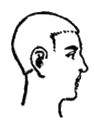
\includegraphics[width=.15\textwidth]{left.jpg}};
      \node (right) [right=4cm  of left] {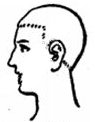
\includegraphics[width=.1\textwidth]{right.jpg}};
      \node (G1) [draw,above=.25cm of left] {Grammar $n$};
      \path[->] (left)  edge[dashed, out=-35,in=215] node[below]  {Data $n$} (right);
      \node (G2) [draw,above=.25cm of right] {Grammar $n+1$};
    \end{tikzpicture}
  \end{center}
	\caption{The process of language acquisition}
	\label{acquisition}
\end{figure}

Yet, while this may be true, it does not necessarily reveal the underlying cause of the change. Crucially, the process of acquisition does not act in a vacuum. The output of one generation serves as the input to the next. And, while this input to acquisition arises from the interplay of many factors, it is not arbitrary. Rather, it is governed by a \emph{pragmatic competence} that ``underlies the ability to use [\emph{grammatical competence}] along with the conceptual system to achieve certain ends or purposes'' \citep[59]{chomsky1980rules}. Or, in Gricean terms, the output from the previous generation arises from the rational use of an internalized grammar. We can visualize this schematically as in Figure \ref{use} where the output of one generation arises through the strategic use of the forms made available by an internalized grammar. Where grammatical competence is formed by a mapping from one generation's \emph{E-Language} to \emph{I-Language} of the next, pragmatic competence is what governs the mapping from each generation's \emph{I-Language} to its \emph{E-Language}.

%the object of study has been taken to be the knowledge of an ideal speaker-hearer in a homogenous speech community \citep{chomsky1965}. 




\begin{figure}
  \begin{center}
    \begin{tikzpicture}
      \node (left)      {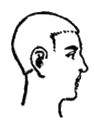
\includegraphics[width=.15\textwidth]{left.jpg}};
      \node (right) [right=4cm  of left] {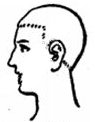
\includegraphics[width=.15\textwidth]{right.jpg}};
      \node (G1) [draw,above=.25cm of left] {Grammar $n$};
      \node (G2) [draw,above=.25cm of right] {Grammar $n$};
      \path[->] (left)  edge[dashed, out=-35,in=220] node[below]  {Data $n$} (right);
      \path[->] (right)  edge[dashed, out=215,in=-40] (left);
    \end{tikzpicture}
  \end{center}
	\caption{The process of language use}
	\label{use}
\end{figure}

Taken together, we can summarize the interaction of these two processes as in Figure \ref{change-labeled}, where both use and acquisition are entwined in the process of change.  So, while we can certainly define change in terms of the internalized grammars of speakers at different points in time, the process of acquisition is not the only locus of change. That is, both the process of externalization, internalization, and the interaction between the two can lead to change in the grammars acquired over time. The central goal of this dissertation is to provide the mathematical tools for defining and analyzing models of change stemming from both use and acquisition. T In doing so, we aim to demonstrate that the notion of pragmatic competence can be integrated into broader theories of change, and is not only incredibly useful but sometimes necessary to explain linguistic change.


\begin{figure}
  \begin{center}
    \begin{tikzpicture}[->,>=stealth',shorten >=1pt,auto,node distance=3.5cm]
      \node (A)      {Grammar $n$};
      \node (B) [below right of=A]  {Data $n$};
      \node (C) [above right of=B] {Grammar $n+1$};
      \node (D) [below right of=C] {Data $n+1$};
      \node (E) [above right of=D] {};
      \path[->] (A)  edge node[sloped, anchor=center, below] {Use} (B)
      (B) edge node[sloped, anchor=center, below] {Acquisition} (C)
      (C) edge[dashed] node {} (D)
      (D) edge[dashed] node {} (E);
    \end{tikzpicture}
  \end{center}
\caption{The iterated process of language change through acquisition and use}
\label{change-labeled}
\end{figure}


At the center of this endeavor will be a diachronic process that implicates both use and acquisition, the development in the expression of sentential negation over time known as \emph{Jespersen's cycle} \citeyearpar{jespersen:1917}. The process is often described as the result of two transitions. The first transition occurs when a preverbal form of negation is replaced by an embracing form, which is initially characterized as being more emphatic. The second transition occurs when this embracing form is subsequently replaced by a purely postverbal form. In the history of English, we observe both of these two transition in Middle English from \emph{\textcolor{red}{ne}} to \emph{\color{blue} ne...not} and from \emph{\color{blue} ne...not}  to \emph{\color{green} not}. Our goal will be to determine the role of use and acquisition in each of these transitions.

In Chapter 2 we begin by distinguishing between two phenomena that have often been conflated in investigations of Jespersen's cycle. In particular, we argue that Jespersen's cycle as it is often described consists of both a \emph{formal} and a \emph{functional cycle}. The formal cycle describes the change in the formal complexity of negation over time. It takes place as negation becomes more and then less formally complex, as can be seen in the transitions in the history of English from \emph{\textcolor{red}{ne}} to \emph{\color{blue} ne...not}  to \emph{\color{green} not}. The functional cycle describes the way that different forms of negation are used to signal meaning. It takes place as one form of plain negation  is replaced by another form. This can be seen in the history of English from \emph{\textcolor{red}{ne}} to \emph{\color{blue} ne...not} where the originally empathic \emph{\color{blue} ne...not} displaces \emph{\textcolor{red}{ne}} as it increases in frequency, loses its emphasis, and comes to signal plain negation. We note the logical and empirical relationship between the two cycles: the functional cycle can occur independently of the formal cycle. This result informs the structure of the rest of the dissertation; we start by addressing the functional cycle before turning to the formal cycle.

The first part of this dissertation addresses the functional cycle. In Chapter 3 we introduce the mathematical tools we will use to model the functional cycle. In particular, we show how we can use evolutionary game theory to describe how meaning is signaled in a population over time. Importantly, these tools allow us to model  a qualified kind of Gricean rationality. That is, individuals are \emph{boundedly rational} insofar as they have limited cognitive and informational resources \citep{simon1955,simon1957}. Yet, these tools allow us to show how the actions of individuals can give rise to change at the population level, even when those small decisions are not the product of conscious deliberation \citep{Keller:1994}. This is particularly important when we turn to the functional cycle in Chapter 4, where we show that the first transition from \emph{\textcolor{red}{ne}} to \emph{\color{blue} ne...not} can be explained as the result of speakers' limitations in keeping track of common versus private knowledge.  So, just as Gricean rationality has been used to explain particular patterns of synchronic use, a kind of bounded rationality allows us to explain the functional cycle. So, how we use these two forms explains why they change over time, and the transition from  \emph{\textcolor{red}{ne}} to \emph{\color{blue} ne...not}. 

However, the same model does not apply to the transition from \emph{\color{blue} ne...not}  to \emph{\color{green} not}, so we turn to the formal cycle in the second part of this dissertation. In Chapter 5 we describe a model of syntactic acquisition and determine its predictions for both of the transitions of the formal cycle. In particular, we show that acquisition cannot explain either of the two transitions from  \emph{\textcolor{red}{ne}} to \emph{\color{blue} ne...not} or  from \emph{\color{blue} ne...not}  to \emph{\color{green} not}, other than as the result of a random change in the grammars acquired. In Chapter 6 we test this possibility using statistical methods developed in population genetics to test for random drift versus selection. We find that we can reject random drift in the case of the first transition from \emph{\textcolor{red}{ne}} to \emph{\color{blue} ne...not}, but we cannot reject drift in the case of the second drift from \emph{\color{blue} ne...not}  to \emph{\color{green} not}. This first result suggests that use is the driving force behind the first transition as part of the functional cycle. The second result shows that acquisition does not play a role in any of the observed transitions.  So, insofar as we can offer an explanation of either of the observed changes, we need the notion of pragmatic competence to do so.

%\section{Language Change}
%
%\begin{itemize}
%	\item Language undoubtedly changes
%	\item Weinreich, Labov, Herzog: constraints but not transition or actuation
%	\item What constitutes change? Mental representations
%\end{itemize}
%
%
%A ..theory" of language change in the rigorous sense can be visualized in a relatively strong form and in a weak form. In its strong form, the theory would predict, from a description of a language state at some moment in time, the course of development which that language would undergo within a specified interval. Few practising historians of language would be rash enough to claim that such a theory is possible. In a more modest version, a theory of language change would merely assert that every language constantly undergoes alteration, and it would formulate constraints on the transition from one state of a language to an immediately succeeding state. It might predict further that no language will assume a form in violation of such formal principles as are postulated to be universal in humnan languages. Without predicting positively what will happen (except that the language will somehow change), such a theory would at least assert that some changes will not take place. WLH p.99
%
%The problem of constraints on immediately succeeding language states, to which we alluded above, is in our view subsumed under the broader theoretical question. Of course, we too want to inquire into the set of possible changes and possible conditions for changes which can take place in a structure of a given type. Nor do we want to dismiss the transition problem: it remains entirely relevant to ask about intervening stages which can be observed, or which must be posited, between any two forms of a language defined for a language community at different times. But if the theory is to be illuminating with respect to recorded histories of languages, we must ask two further questons: How are the observed changes embedded in the matrix of linguistic and extralinguistic concomitants of the forms in question? (That is, what other changes are associated with the given changes in
%a manner that cannot be attributed to chance?) And how can the observed changes be evaluated in terms of their effect upon linguistic structure, upon communicative efficiency (as related, e.g., to functional load), and on the wide range of nonrepresentational factors involved in speaking? WLH p.101
%
%\section{Linguistic Explanation}
%
%\begin{itemize}
%	\item Causality : necessary and sufficient conditions
%	\item What counts as an explanation?
%	\item Chomsky: Observational, Descriptive, Explanatory adequacy (Van Frassen: Deductive)
%	\item Description alone is not enough!
%	\item What counts as an explanation in Linguistics?
%\end{itemize}
%
%\section{Causal Forces}
%
%\begin{itemize}
%	\item Need additional evidence that description is grounded in reality somehow.
%	\item We can't rewind and redo language experiments!
%	\item We can note the falsifying cases
%%	\item Stochastic vs deterministic processes
%%	\item Mean dynamics
%\end{itemize}
%
%Languages change. 
%
%Or rather, the mental representations that characterize knowledge change. Somewhere along the iterated chain of language transmission, from one generation to the next, the content of what is learned is substantially different. 
%
%Language change is evidenced by a difference between the linguistic expressions of one generation and the next. Given that the output from one generation serves as the input to the next, both language acquisition and use are crucial to the process of change. While the input to acquisition arises from the interplay of many factors, it is not arbitrary. Rather, it is governed by a \emph{pragmatic competence} that ``underlies the ability to use [\emph{grammatical competence}] along with the conceptual system to achieve certain ends or purposes'' \citep[59]{chomsky1980rules}. In the terms of \cite{chomsky1986knowledge}, the process of language acquisition maps the \emph{E-Language} of one generation to the \emph{I-Language} of the next, whereas pragmatic competence is what governs the mapping from each generation's \emph{I-Language} to its \emph{E-Language}.
%
%In the Gricean tradition \citep{Grice:1975,Levinson:1983, Horn:1984}, this pragmatic competence has been framed in terms of speakers' beliefs, preferences, and intentions. Linguistic expressions are used according to a \emph{Cooperative Principle} whereby interlocutors are taken to make the appropriate contribution to the conversation at the appropriate time towards ``the accepted purpose or direction of the talk exchange'' \citep[26]{Grice:1975}. This framework deftly captures the systematic relationship between what is \emph{said} and what is \emph{meant}, but is clearly an idealization: speakers and hearers might, but need not have the same preferences or goals in a given exchange.   This dissertation aims at understanding the consequences of loosening the assumption of Gricean commonality. It will examine how differences in speakers' and hearers' preferences might impact the use and acquisition of linguistic signals over time. 
%
%At the center of this endeavor will be a diachronic process that implicates both use and acquisition, the development in the expression of negation over time known as \emph{Jespersen's Cycle} \citeyearpar{jespersen:1917}. The main components of this dissertation address the main components of the cycle in turn. First, we consider how the expression of negation transitions from a purely preverbal negator with an optional \emph{emphatic} postverbal element towards a system with obligatory preverbal and postverbal elements. We present a formal model that derives this transition from even a slight preference for exaggeration on the part of speakers. If speakers prefer hearers' response to the emphatic form, then the optional postverbal element will increase in use. On the way up it experiences a kind of \emph{rhetorical devaluation} \citep{dahl:2001}, and is at least partially \emph{bleached} of its emphatic force because, simply put, to ``to emphasize everything is to emphasize nothing'' \citep{kiparsky-condoravdi:2006}. Second, we consider how the expression of negation can shift from the original preverbal negator to the new, increasingly-used, postverbal element. We outline the conditions under which a learner would posit that the postverbal element is a negator in its own right. If the preverbal element appears in contexts where it does not itself express negation, this provides evidence that postverbal element expresses negation and for the eventual loss of the preverbal element entirely. We consider the interaction between these two components of the cycle.
%
%The main contributions of this line of research are the following. First,  it extends recent work in game-theoretic pragmatics that has begun to explore the broader space of possibly divergent preferences \citep{benz-jager-van-rooij:2006, franke:2008, franke-etal:2012, de-jaegher-van-rooij:2013}. This can be taken as a straightforward generalization of the Gricean program to understand the use of linguistic expressions not just as something ``all or most do \emph{in fact} follow but as something that it is \emph{reasonable} for us to follow, that we \emph{should not} abandon'' \citep[29]{Grice:1975}.  Second, it incorporates this perspective into the use of linguistic signals over time. In particular, it suggests how Grice's criterion of reasonability might cut both ways: there are some patterns of use that we \emph{should} and \emph{do} abandon. Differentiating the cases where we expect stability from those where we expect change adds to a broader causal theory of language change \citep{yang2000internal}. 
%
%
%Namely, it offers an additional \emph{internal} force of language change, which derives from a shared pragmatic competence. In the case of Jespersen's Cycle it suggests how morphosyntactic change might arise through a kind of communicative bleaching.   More broadly, it offers insight into the interaction between use and acquisition implicit in the common representation of iterated language change as in Figure \ref{trans}.
%
%\begin{figure}
%\begin{center}
%\begin{tikzpicture}[->,>=stealth',shorten >=1pt,auto,node distance=3cm]
%  \node (A)      {Grammar $n$};
%  \node (B) [below right of=A]  {Data $n$};
%  \node (C) [above right of=B] {Grammar $n+1$};
%  \node (D) [below right of=C] {Data $n+1$};
%  \node (E) [above right of=D] {};
%\path[->] (A)  edge node {} (B)
%  (B) edge node {} (C)
%  (C) edge node {} (D)
%  (D) edge[dashed] node {} (E);
%\end{tikzpicture}
%\end{center}
%\caption{The iterated process of language change through acquisition and use}
%%\label{trans}
%\end{figure}
%
%
%\begin{figure}
%  \begin{center}
%    \begin{tikzpicture}
%      \node (left)      {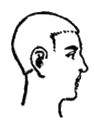
\includegraphics[width=.15\textwidth]{left.jpg}};
%      \node (right) [right=4cm  of left] {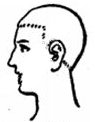
\includegraphics[width=.1\textwidth]{right.jpg}};
%      \node (G1) [draw,above=.25cm of left] {Grammar $n$};
%      \path[->] (left)  edge[dashed, out=-35,in=215] node[below]  {Data $n$} (right);
%      \node (G2) [draw,above=.25cm of right] {Grammar $n+1$};
%    \end{tikzpicture}
%  \end{center}
%	\caption{}
%%	\label{acquisition}
%\end{figure}
%
%
%\begin{figure}
%  \begin{center}
%    \begin{tikzpicture}
%      \node (left)      {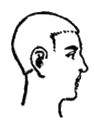
\includegraphics[width=.15\textwidth]{left.jpg}};
%      \node (right) [right=4cm  of left] {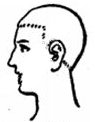
\includegraphics[width=.15\textwidth]{right.jpg}};
%      \node (G1) [draw,above=.25cm of left] {Grammar $n$};
%      \node (G2) [draw,above=.25cm of right] {Grammar $n$};
%      \path[->] (left)  edge[dashed, out=-35,in=220] node[below]  {Data $n$} (right);
%      \path[->] (right)  edge[dashed, out=215,in=-40] (left);
%    \end{tikzpicture}
%  \end{center}
%	\caption{}
%	\label{use}
%\end{figure}
%
%
%\begin{figure}
%  \begin{center}
%    \begin{tikzpicture}[->,>=stealth',shorten >=1pt,auto,node distance=3cm]
%      \node (A)      {Grammar $n$};
%      \node (B) [below right of=A]  {Data $n$};
%      \node (C) [above right of=B] {Grammar $n+1$};
%      \node (D) [below right of=C] {Data $n+1$};
%      \node (E) [above right of=D] {};
%      \path[->] (A)  edge node[sloped, anchor=center, below] {Use} (B)
%      (B) edge node[sloped, anchor=center, below] {Acquisition} (C)
%      (C) edge[dashed] node {} (D)
%      (D) edge[dashed] node {} (E);
%    \end{tikzpicture}
%  \end{center}
%\caption{The iterated process of language change through acquisition and use}
%\label{change-labeled}
%\end{figure}
%
%
%
%
%
%The rest of the proposal is structured as follows. Section \ref{Background} offers an overview of Jespersen's Cycle.  We consider the two major approaches to the change, as a \emph{pull-chain} or a \emph{push-chain}. We adopt the latter given that the driving force behind the cycle appears to be pragmatic in nature, stemming from continuous loss and renewal of emphatic negation. We then consider a natural simplification of Eckardt's \citeyear{eckardt2006} analysis of emphatic negation. In Section \ref{Signaling} we develop the mathematical framework that will be used to explicitly connect the analysis of emphatic negation with the cycle. In Section \ref{Cycles} we apply the framework and consider the cycle as a signaling game played in a population where the interests of speakers and hearers slightly diverge. We determine the conditions for the existence of different kinds of equilibria, and the impact of the introduction of new signals under the game dynamics. Finally, in Section \ref{Stability} we 
%determine how the change brought about by use might impact acquisition over time. We suggest different mechanisms that might impact the amount of evidence available to learners at various points in time and how this shapes the trajectory of the change.
%
%\begin{quote}
%	   I am, however, enough of a rationalist to want to find a basis that underlies these facts, undeniable though they may be; I would like to be able to think of the standard type of conversational practice not merely as something that all or most do \textbf{in fact} follow but as something that it is \textbf{reasonable} for us to follow, that \textbf{we should not abandon}. 
% \end{quote}           
%
%\begin{quote}
%As one of my avowed aims is to see talking as a special case or variety of purposive, indeed rational, behaviour, it may be worth noting that the specific expectations or presumptions connected with at least some of the foregoing maxims have their analogues in the sphere of transactions that are not talk exchanges. (Grice 1989, p. 28)
%\end{quote}
%
%\begin{quote}
%[T]o say what a word means in a language is to say what
%it is in general optimal for speakers of that language to
%do with that word, or what use they are to make of it;
%what particular intentions on particular occasions it is
%proper for them to have. Of course, there is no
%suggestion that they always have to have those
%intentions: it would merely be optimal, ceteris paribus,
%for them to have them. (Grice, 1989, p. 299)
%\end{quote}
%
%\begin{quote}
%The maxims do not seem to be coordinate. The maxim
%of Quality [...] does not seem to be just one among a
%number of recipes for producing contributions; it seems
%rather to spell out the difference between something�s
%being, and (strictly speaking) failing to be, any kind of
%contribution at all. False information is not an inferior
%kind of information; it just is not information. (Grice,
%1989, p.371)
%\end{quote}
%
%Conflicts of interest play markedly different roles in Linguistics and Biology. On the one hand, Gricean pragmatics has aimed at understanding the inferences that a listener can draw from a speaker's contribution on the explicit assumption of a shared set of purposes for an exchange. On the other hand, animal signaling has aimed at understanding the existence and persistence of signaling systems in the face of varying degrees of inter- and intra-species conflict.  Both endeavors hinge on the role of conflict, either in its presence or absence. Yet, in the abstract, both deal with the transmission and interpretation of signals. This leads us to consider what happens when we extend our linguistic considerations beyond perfectly aligned interests. 
%
%At first glance, this step outside the idealized realm of common causes yields some forbidding results: conflicts of interest erode communication. The following reasoning, familiar from biological studies of animal signaling, makes clear the root of this unraveling \citep{searcy-nowicki:2005}. Imagine two agents: a sender who sends a signal and a receiver who receives the signal. Suppose that the sender has no incentive to be truthful, in fact, let us suppose that he has every incentive to deceive the receiver. If the sender has an incentive to deceive, then the receiver should not listen. If the receiver does not listen, then the sender has no motive to signal in the first place. Crucially, the actions of the sender depend on those of the receiver and vice versa. Given this interdependence, conflicting interests undermine the information conveyed by signals, rendering them, so to speak, meaningless. 
%
%The same reasoning holds in the case of an entire population of senders and receivers interacting over time. Senders will learn or evolve to dissimulate and receivers will learn or evolve to distrust. This process takes on the familiar form of the \emph{tragedy of the commons} \citep{hardin:1968}. Individuals will always be tempted to exploit the common resource of credulity. Collectively, this incentive to exploit exhausts the resource. Only a fool would tell the truth when there is something to be gained from deception, and only a fool would trust others to be truthful. 
%
%
%\begin{quote}
%	   Make your conversational contribution  such as is required, at the stage at which it occurs, by the accepted purpose or direction of the talk exchange in which you are engaged. One might label this the \textbf{Cooperative Principle}.
%\end{quote}           
%
%
%Silence, or at best meaningless babble, is the equilibrium state in the population: neither senders nor receivers have reason to unilaterally change their behavior. Thomas Schelling's grim pronouncement comes to mind \citep[26]{schelling:1978}:  
%
%\begin{quote}
% The body of a hanged man is in equilibrium when it finally stops swinging, but
%nobody is going to insist that the man is all right.
%\end{quote}
%This sentiment holds doubly. Not only is the inability to convey information problematic, but, we do actually observe informative signaling. The existence of such signaling despite conflicting interests is a genuine puzzle. 
%
%This problem was not lost on Grice, insofar as he recognized the fundamental
%role of his \emph{Maxim of Quality} to the entire enterprise.
%
%\begin{quotation}
%It is obvious that the observance of some of these maxims is a matter of less urgency than is the observance of others; a man who has expressed himself with undue prolixity would, in general, be open to milder comment than would a man who has said something he believes to be false...[O]ther maxims come into operation only on the assumption that this maxim of Quality is satisfied \citep[27]{Grice:1975}
%\end{quotation}
%
%Yet, while we have every incentive to abide by the maxim of Quality when it serves our interests, we have every reason to do otherwise when it does not. So, what keeps human language from the downward spiral to silence? In this regard we can look to animal communication where much work has been devoted to explaining the evolutionary stability of communication. In large part, these solutions take the form of different mechanisms that mitigate conflicts of interest between senders and receivers. 
%
%For example, a sender might guarantee his commitment to the truth by incurring a sufficiently high cost to send a signal. This \emph{handicap principle}  \citep{Zahavi:1975} allows for stable signaling despite conflicting interests.\footnote{See \cite{maynard-smith-harper:2004} and \cite{searcy-nowicki:2005} for thorough discussions of handicaps in animal signaling. Also,\cite{grose:2011} offers a concise but useful discussion of the history and details of the handicap principle. In the economic tradition, \cite{spence:1973} develops a parallel model for educational attainment as a costly signal of job suitability.} To take the usual example, a peacock incurs a cost for his magnificent tail: significant metabolic resources are required to develop the tail, and once developed, his ability to fly is hampered and it makes him more conspicuous to predators. But, successfully bearing the tail serves as a signal of his genetic worth. A weaker peacock would not have been able to support the tail and avoid becoming 
%something else's lunch. Thus, potential mates  can take the tail as a signal of a a truly fit peacock. 
%
%When we turn our attention to language, this sort of mechanism need not be appropriate.  In fact, the notion that truthfulness is enforced by cost is problematic: truth tellers expend as much effort learning and producing their language as liars, and no more. As we say, talk is cheap. There are, of course, various alternatives to handicaps that are appropriate for the case of language \citep{scott-phillips:2008}. A particularly appealing alternative given the social nature of humans, and language, is that of reputation. The minimal requirements for a reputation are the ability of agents to recognize each other individually, keep track of past interactions, and condition future behavior on the outcome of those interactions \citep{Trivers1971}. In the long run, the immediate benefits of deception might not be worth the consequences of a bad reputation.
%
%Abstracting away from the details of the actual mechanisms that mitigate conflict, we can consider three general questions.  First, how effective are these mechanisms in aligning the interests of senders and receivers? Given that language exists, such mechanisms are clearly sufficient to stave off total collapse. However, given that signals are not always used in accordance with the Maxim of Quality, such mechanism are not sufficient to ensure the idealized case of Gricean commonality. Second, if language is indeed subject to a host of competing pressures, what impact will this have on how linguistic signals are used over time?  If not a tragedy of the commons, might we find a lesser \emph{tragedy of the conversation} where particular signals, but not the system as a whole, are destabilized? Third, do we find instantiations of the predicted patterns of language use? In what follows, these second two question will be our chief concern. 
%
%\section{Roadmap}
%
%\begin{enumerate}
%	\item In Chapter \ref{jespersens-cycle} we outline....
%	\item In Chapter \ref{evolutionary-game-theory} we...
%	\item In Chapter \ref{Cycles} we ...
%	\item in Chapter \ref{learning-theory} we...
%	\item in Chapter \ref{Stability}
%	\item in Chapter \ref{conclusion} we summarize our results.
%\end{enumerate}�


